\documentclass{article}

\usepackage[
  paperwidth=16.438in,
  paperheight=11.75in,
  margin=0in
]{geometry}
\usepackage{fontspec}
\usepackage{graphicx}
\usepackage{xcolor}
\usepackage{tikz}

\setmainfont{Libertinus Serif}
\pagestyle{empty}
\setlength{\parindent}{0pt}

\definecolor{coverwhite}{HTML}{F3F0E8}
\definecolor{covergold}{HTML}{D9B878}
\definecolor{coverblue}{HTML}{AFC9E7}
\definecolor{covernavy}{HTML}{07111F}

\begin{document}
\begin{tikzpicture}[remember picture,overlay]
  % Full-wrap artwork, including the 0.625-inch outer wrap area.
  \node[anchor=south west,inner sep=0pt] at (current page.south west) {%
    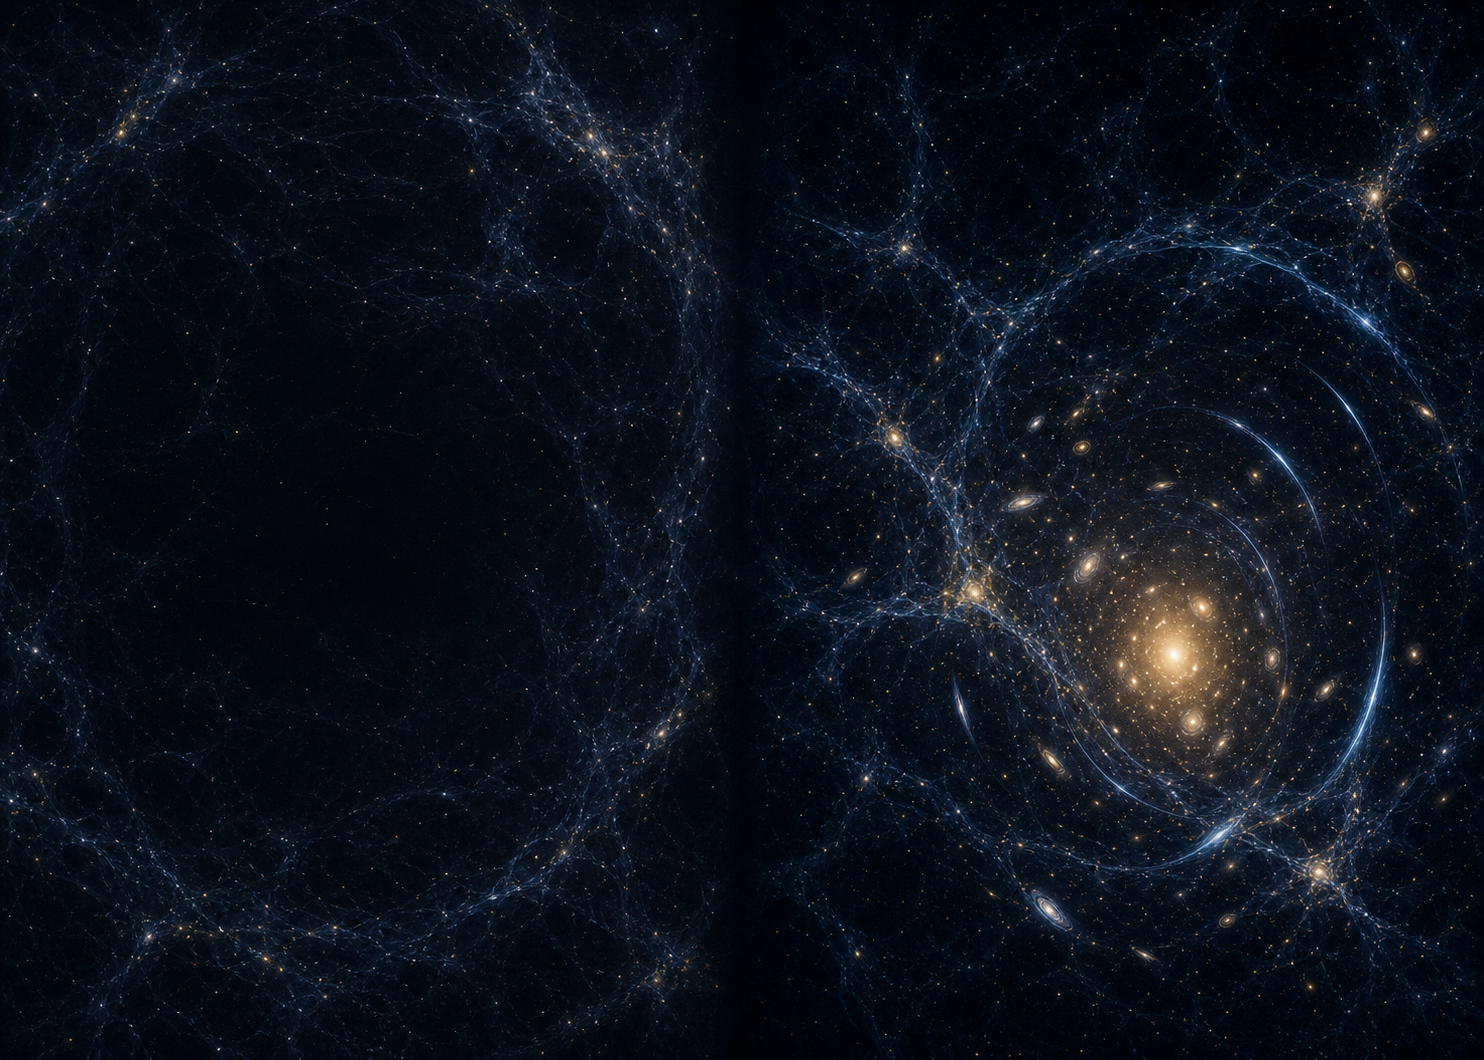
\includegraphics[
      width=16.438in,
      height=11.75in
    ]{cover-wrap-background.png}%
  };

  % Quiet tonal fields behind copy; kept translucent so the cosmic web remains.
  \fill[covernavy,opacity=0.63]
    ([xshift=0.90in,yshift=1.10in]current page.south west)
    rectangle
    ([xshift=7.55in,yshift=10.70in]current page.south west);
  \fill[covernavy,opacity=0.22]
    ([xshift=8.80in,yshift=1.10in]current page.south west)
    rectangle
    ([xshift=15.55in,yshift=10.70in]current page.south west);
  \fill[covernavy,opacity=0.46]
    ([xshift=7.875in]current page.south west)
    rectangle
    ([xshift=8.563in]current page.north west);

  % Back cover copy. The lower-right barcode zone is intentionally empty.
  \node[
    anchor=north west,
    text=coverwhite,
    text width=5.35in,
    align=left,
    inner sep=0pt
  ] at ([xshift=1.25in,yshift=-1.35in]current page.north west) {%
    {\fontsize{16}{19}\selectfont\scshape
      Distribution of Matter in the Universe\par}
    \vspace{0.25in}
    {\color{covergold}\rule{0.90in}{0.7pt}\par}
    \vspace{0.25in}
    {\fontsize{11.2}{15.2}\selectfont
      The distribution of matter preserves a record of the composition,
      evolution, and structure of the Universe. This dissertation studies that
      distribution in two complementary regimes: gravitationally bound galaxy
      clusters and the cosmic large-scale structure.\par
      \vspace{0.17in}
      Through strong and weak gravitational lensing, non-parametric mass
      reconstruction, lensing time delays, and models of the matter power
      spectrum, the work connects observations of individual clusters to the
      statistical description of cosmic structure. It examines mass--galaxy
      offsets, dark-matter substructure, baryonic effects on cosmological
      measurements, and the reconstructed mass maps of Hubble Frontier Field
      clusters.\par
      \vspace{0.17in}
      The five research studies collected here show how lensing clusters and
      large-scale structure provide distinct but mutually reinforcing views of
      the matter content of the Universe.\par}
    \vspace{0.34in}
    {\fontsize{9.2}{12}\selectfont\color{coverblue}
      COSMOLOGY \quad GRAVITATIONAL LENSING \quad DARK MATTER\par
      LARGE-SCALE STRUCTURE \quad GALAXY CLUSTERS\par}
  };

  \node[
    anchor=south west,
    text=coverwhite,
    text width=2.55in,
    align=left,
    inner sep=0pt
  ] at ([xshift=1.25in,yshift=1.18in]current page.south west) {%
    {\fontsize{9.5}{12.5}\selectfont
      Irshad Mohammed\\
      University of Zurich\\
      Doctor of Natural Sciences, 2015\par}
  };

  % Front cover.
  \node[
    anchor=north west,
    text=coverwhite,
    text width=5.85in,
    align=left,
    inner sep=0pt
  ] at ([xshift=9.25in,yshift=-1.30in]current page.north west) {%
    {\fontsize{27}{31}\selectfont\bfseries\scshape
      Distribution of Matter\\
      in the Universe\par}
    \vspace{0.25in}
    {\color{covergold}\rule{1.15in}{0.8pt}\par}
    \vspace{0.23in}
    {\fontsize{14}{18}\selectfont\itshape
      From Lensing Clusters\\
      to Large-Scale Structure\par}
  };

  \node[
    anchor=south west,
    text=coverwhite,
    inner sep=0pt
  ] at ([xshift=9.25in,yshift=1.32in]current page.south west) {%
    {\fontsize{15}{18}\selectfont\scshape Irshad Mohammed}
  };

  % Spine: 0.688 inches wide, centered between the two 7.25-inch trim panels.
  \node[
    rotate=-90,
    text=coverwhite,
    inner sep=0pt
  ] at ([xshift=8.219in,yshift=5.875in]current page.south west) {%
    {\fontsize{12.5}{14}\selectfont\scshape
      Distribution of Matter in the Universe
      \quad{\color{covergold}\textperiodcentered}\quad
      Irshad Mohammed}
  };
\end{tikzpicture}
\null
\end{document}
